\chapter{Methodology}
\label{chap:methodology}
This chapter outlines the methodology that offers a unique framework for users to experiment with multiple loss functions, combining them and applying several merging strategies to output a final loss. The goal is to enable users to gain insights into the most suitable combination for their specific data. The chapter is organized into two sections. The \nameref{sec:limiting_factors} section expands upon the constraints of the \acf{DL} as mentioned earlier, incorporating additional limitations and summarizing them to lay the groundwork for the subsequent section. In section \nameref{sec:loss_merging}, a framework is introduced that facilitates combining and merging multiple loss functions to address the discussed limitations and enhance the performance compared to models trained with individual loss functions.

\begin{figure}[H]%[htbp]
  \centering
  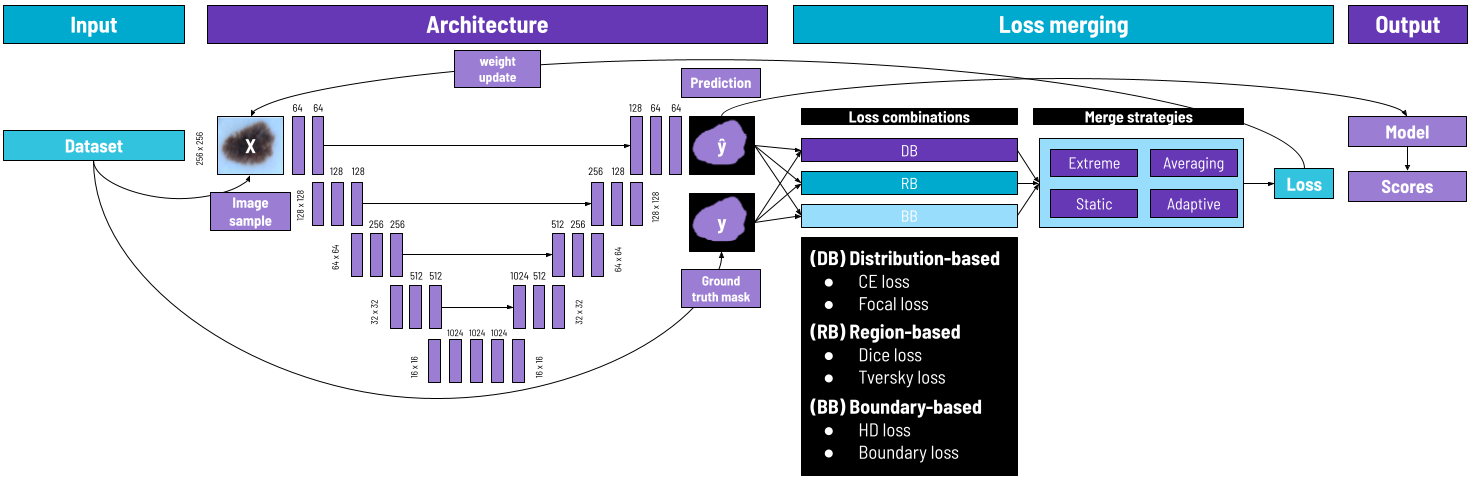
\includegraphics[width=\imgWidthXL]{images/Pipeline_white_bg.png}
  \caption[Proposed segmentation framework]{Illustration of the proposed framework where individual losses originating from distribution, region, or boundary-based types are generated in each training iteration. These losses are combined and merged using various proposed strategies, resulting in a single, unified loss. This approach aims to enhance performance beyond that of baseline models, which are trained with just a single loss function.}
  \label{framework}
\end{figure}

\section{Limiting Factors}
\label{sec:limiting_factors}
This section extends the taxonomy introduced by \cite{9338261} for the \ac{DL}, addressing the following limitations for the six loss functions introduced in \secref{subsec:segmentation_objectives}.
\begin{enumerate}
  \item \textbf{Distance insensitivity:} As previously discussed in the context of the \acf{DL}, insensitivity to distances is a notable limitation for a range of loss functions. Among the functions covered in \secref{subsec:segmentation_objectives}, all distribution and region-based functions exhibit this limitation. For distribution-based functions, this limitation can be demonstrated analogously to what is shown for \ac{DL} in \figref{dice_limit_1}. However, this insensitivity does not constrain boundary-based loss functions that incorporate a distance transform in their calculations. See the corresponding row of table \ref{tab:limitation_quantitative_results} for quantitative analysis.
  \item \textbf{Boundary insensitivity:} This limitation, initially introduced in \chapref{chap:literature_review} for the \ac{DL}, is also pertinent to distribution and region-based loss functions. The two boundary-based loss functions, namely \ac{HL} and \ac{BL}, appear to be somewhat resilient to this limitation, although they are not completely aware of the entire shape. In instances where two predictions are compared - with the first matching the shape of the ground truth but located farther away than a second prediction that exhibits a different shape - the latter might yield a smaller loss, thereby providing possible misleading feedback. As demonstrated in table \ref{tab:limitation_quantitative_results}, distribution and region-based losses yield the same result.
  \item \textbf{Region-size sensitivity:} This sensitivity is associated with the issue of class imbalance and predominantly affects distribution and region-based loss functions. While initially introduced in the context of \ac{DL} in \chapref{chap:literature_review}, distribution-based loss functions are known to work best on data with equal distribution and thus are also affected by sensitivity to region size \cite{Jadon_2020} \cite{YEUNG2022102026} while boundary-based loss functions are not affected by this type of sensitivity. Table \ref{tab:limitation_quantitative_results} presents a quantitative analysis where distribution and region-based losses change substantially comparing $l_1$ with $l_2$ where the former represents one misclassified pixel on large regions while the latter stems from one misclassified pixel on small regions.
  \item \textbf{FP / FN weight insensitivity:} All loss functions, with the exception of the \acf{TL}, which is explicitly designed to address this issue, exhibit insensitivity to the weighting of false positives and false negatives. As highlighted in \secref{subsec:segmentation_metrics}, researchers may desire to manipulate high precision, low recall scenarios, or vice versa, depending on specific objectives. This manipulation can be achieved by manually adjusting the weights attributed to false positives or false negatives. On table \ref{tab:limitation_quantitative_results} we can see that the \ac{TL} is the only function sensitive to FP / FN weight.
  \item \textbf{Outlier sensitivity:} Outliers can be described as data points unusually distant from the overall pattern and deviate significantly from other observations. Outliers may arise for various reasons, such as errors in labeling or the presence of noise. In the context of loss functions discussed in \secref{subsec:segmentation_objectives}, it is essential to note that all loss functions can be sensitive to outliers. This sensitivity can disproportionately affect the model's total loss value during training. While it is generally difficult to ascertain which loss function is most affected by outliers, it is observed that boundary-based loss functions are more impacted when the mislabeled pixels are further from the region of interest. Conversely, region-based loss functions are influenced equally by pixels closer to or further from the region of interest. While many techniques exist, such as data augmentation and regularization, which can mitigate the impact of outliers and enhance the model's performance. For a more comprehensive understanding of this subject, please refer to \cite{Cho_2023_WACV}, \cite{DBLP:journals/corr/abs-1802-09129}, \cite{bevandi2019simultaneous}.
  \item \textbf{Computational complexity:} Boundary-based loss functions are known to be computationally expensive since they involve distance calculations between sets of points, which are much more complex and time-consuming compared to other loss functions \cite{Kervadec_2021}. To reduce the complexity of the \ac{HL} function, the one-sided version $HL_{os}$ can be used instead, as defined in \ref{eq:one_sided_hd}, to reduce the effort of the distance transform $D_y(i,j)$, as defined in \ref{eqn:distance_transform_y}, for the ground truth only. Since $D_y(i,j)$ does not change during training, it can be pre-calculated for all output labels $Y$ whenever the model is initialized. Similarly, the \ac{BL} function presented in \secref{subsec:segmentation_objectives} also requires the distance transformation to be pre-calculated, which can cause a bottleneck, especially for high-resolution images. To further reduce computational complexity, a subsampling method can use only a subset of points instead of all the pixels in the image.
  \item \textbf{Manual parameter tuning:} Manual hyperparameter tuning can be a limiting factor for loss functions. Hyperparameter search can be time-consuming, especially when dealing with large datasets or complex architectures. It may also require domain expertise related to the dataset or the clinical operation, as discussed in \secref{subsec:tversky}. Additionally, hyperparameter search only sometimes guarantees to find the best solution since it relies on the intuition or experience of the user. To improve manual tuning and increase the likelihood of finding an optimal set of values, techniques such as grid search \cite{9504761}, random search \cite{10.5555/2188385.2188395}, Bayesian optimization \cite{WU201926}, or evolutionary algorithms \cite{DBLP:journals/corr/abs-2105-09821} can be used. These techniques automate the hyperparameter search process and can save time and resources.
\end{enumerate}
The following table \ref{tab:limitation_quantitative_results} presents the quantitative results for limitations 1 through 4 confirming each statement from above. Each loss column displays two results, $l_1$ and $l_2$, which correspond to specific combinations of $y$ and $\hat{y}$, as previously discussed in the context of \acf{DL} in \chapref{chap:literature_review}. The results that are underlined indicate scenarios that are either not affected or less affected by the corresponding limitation.

% Please add the following required packages to your document preamble:
% \usepackage{graphicx}
% \usepackage[table,xcdraw]{xcolor}
% If you use beamer only pass "xcolor=table" option, i.e. \documentclass[xcolor=table]{beamer}
% \usepackage[normalem]{ulem}
% \useunder{\uline}{\ul}{}
\begin{table}[H]
  \centering
  \resizebox{\textwidth}{!}{%
  \begin{tabular}{l|cccc|cccc|cccc|l}
  \cline{2-13}
   &
    \multicolumn{4}{c|}{\cellcolor[HTML]{6638B6}{\color[HTML]{FFFFFF} \textbf{DB}}} &
    \multicolumn{4}{c|}{\cellcolor[HTML]{00A9CE}{\color[HTML]{FFFFFF} \textbf{RB}}} &
    \multicolumn{4}{c|}{\cellcolor[HTML]{99DDFD}{\color[HTML]{FFFFFF} \textbf{BB}}} &
     \\ \cline{2-13}
   &
    \multicolumn{2}{c|}{\cellcolor[HTML]{000000}{\color[HTML]{FFFFFF} CE}} &
    \multicolumn{2}{c|}{\cellcolor[HTML]{000000}{\color[HTML]{FFFFFF} FL}} &
    \multicolumn{2}{c|}{\cellcolor[HTML]{000000}{\color[HTML]{FFFFFF} DL}} &
    \multicolumn{2}{c|}{\cellcolor[HTML]{000000}{\color[HTML]{FFFFFF} TL}} &
    \multicolumn{2}{c|}{\cellcolor[HTML]{000000}{\color[HTML]{FFFFFF} BL}} &
    \multicolumn{2}{c|}{\cellcolor[HTML]{000000}{\color[HTML]{FFFFFF} HL}} &
    \multicolumn{1}{c}{} \\ \cline{2-14} 
   &
    \multicolumn{1}{c|}{$l_1$} &
    \multicolumn{1}{c|}{$l_2$} &
    \multicolumn{1}{c|}{$l_1$} &
    $l_2$ &
    \multicolumn{1}{c|}{$l_1$} &
    \multicolumn{1}{c|}{$l_2$} &
    \multicolumn{1}{c|}{$l_1$} &
    $l_2$ &
    \multicolumn{1}{c|}{$l_1$} &
    \multicolumn{1}{c|}{$l_2$} &
    \multicolumn{1}{c|}{$l_1$} &
    $l_2$ &
    \multicolumn{1}{c|}{Reference} \\ \hline
  \multicolumn{1}{|l|}{\cellcolor[HTML]{9B7DD4}{\color[HTML]{FFFFFF} Distance Insensitivity}} &
    \multicolumn{1}{c|}{8.16} &
    \multicolumn{1}{c|}{8.16} &
    \multicolumn{1}{c|}{8.15} &
    8.15 &
    \multicolumn{1}{c|}{1.00} &
    \multicolumn{1}{c|}{1.00} &
    \multicolumn{1}{c|}{\cellcolor[HTML]{FFFFFF}0.67} &
    \cellcolor[HTML]{FFFFFF}0.67 &
    \multicolumn{1}{c|}{\cellcolor[HTML]{FFFFFF}{\ul 0.04}} &
    \multicolumn{1}{c|}{\cellcolor[HTML]{FFFFFF}{\ul 0.08}} &
    \multicolumn{1}{c|}{\cellcolor[HTML]{FFFFFF}{\ul 0.15}} &
    \cellcolor[HTML]{FFFFFF}{\ul 0.39} &
    \multicolumn{1}{l|}{\figref{dice_limit_1}} \\ \hline
  \multicolumn{1}{|l|}{\cellcolor[HTML]{9B7DD4}{\color[HTML]{FFFFFF} Boundary insensitivity}} &
    \multicolumn{1}{c|}{6.36} &
    \multicolumn{1}{c|}{6.36} &
    \multicolumn{1}{c|}{6.35} &
    6.35 &
    \multicolumn{1}{c|}{0.40} &
    \multicolumn{1}{c|}{0.40} &
    \multicolumn{1}{c|}{\cellcolor[HTML]{FFFFFF}0.33} &
    \cellcolor[HTML]{FFFFFF}0.33 &
    \multicolumn{1}{c|}{\cellcolor[HTML]{FFFFFF}0.04} &
    \multicolumn{1}{c|}{\cellcolor[HTML]{FFFFFF}0.04} &
    \multicolumn{1}{c|}{\cellcolor[HTML]{FFFFFF}{\ul 0.15}} &
    \cellcolor[HTML]{FFFFFF}{\ul 0.18} &
    \multicolumn{1}{l|}{\figref{dice_limit_2}} \\ \hline
  \multicolumn{1}{|l|}{\cellcolor[HTML]{9B7DD4}{\color[HTML]{FFFFFF} Region-size sensitivity}} &
    \multicolumn{1}{c|}{0.32} &
    \multicolumn{1}{c|}{1.68} &
    \multicolumn{1}{c|}{0.32} &
    1.68 &
    \multicolumn{1}{c|}{0.03} &
    \multicolumn{1}{c|}{0.14} &
    \multicolumn{1}{c|}{\cellcolor[HTML]{FFFFFF}0.04} &
    \cellcolor[HTML]{FFFFFF}0.15 &
    \multicolumn{1}{c|}{\cellcolor[HTML]{FFFFFF}{\ul 0.01}} &
    \multicolumn{1}{c|}{\cellcolor[HTML]{FFFFFF}{\ul 0.01}} &
    \multicolumn{1}{c|}{\cellcolor[HTML]{FFFFFF}{\ul 0.04}} &
    \cellcolor[HTML]{FFFFFF}{\ul 0.04} &
    \multicolumn{1}{l|}{\figref{dice_limit_3}} \\ \hline
  \multicolumn{1}{|l|}{\cellcolor[HTML]{9B7DD4}{\color[HTML]{FFFFFF} FP / FN weight insensitivity}} &
    \multicolumn{1}{c|}{1.68} &
    \multicolumn{1}{c|}{1.68} &
    \multicolumn{1}{c|}{1.68} &
    1.68 &
    \multicolumn{1}{c|}{0.14} &
    \multicolumn{1}{c|}{0.14} &
    \multicolumn{1}{c|}{\cellcolor[HTML]{FFFFFF}{\ul 0.07}} &
    \cellcolor[HTML]{FFFFFF}{\ul 0.14} &
    \multicolumn{1}{c|}{\cellcolor[HTML]{FFFFFF}0.01} &
    \multicolumn{1}{c|}{\cellcolor[HTML]{FFFFFF}0.01} &
    \multicolumn{1}{c|}{\cellcolor[HTML]{FFFFFF}0.04} &
    \cellcolor[HTML]{FFFFFF}0.04 &
    \multicolumn{1}{l|}{\figref{dice_limit_4}} \\ \hline
  \end{tabular}%
  }
  \caption{Results demonstrating limitation no. 1 to 4 for six loss functions quantitatively.}
  \label{tab:limitation_quantitative_results}
  \end{table}

\subsection{Summary}
Table \ref{tab:limiting_factors} summarizes the impact of each limiting factor on the six loss functions presented. It reveals that \ac{HL} and \ac{BL} are less affected by distance insensitivity, boundary insensitivity, and region-size sensitivity compared to the other loss functions. However, boundary-based loss functions have drawbacks, such as computational complexity, instability, and complex implementations.

Finding a single loss function that entirely circumvents all limitations is challenging. Nonetheless, the subsequent chapter explores a set of combinations of loss functions and merging techniques to leverage the individual strengths of each loss function to generate a more precise learning signal, thereby enhancing performance. This improvement can be important in various fields requiring a highly accurate segmentation performance, including distance measurements.

Although various implementations have attempted to address some of these limitations, such as the \ac{TL}, proposed by \cite{DBLP:journals/corr/SalehiEG17a}, which tackles the FP/FN weight insensitivity or the \ac{GDL} from \cite{Sudre_2017}, which is capable of handling region-size insensitivity there is an absence of a unified framework that systematically combines and analyzes a set of loss functions. To the best of the author's knowledge, such a unified, comprehensive approach is yet to be developed.
% Please add the following required packages to your document preamble:
% \usepackage{multirow}
% \usepackage{graphicx}
% \usepackage[table,xcdraw]{xcolor}
% If you use beamer only pass "xcolor=table" option, i.e. \documentclass[xcolor=table]{beamer}
\begin{table}[H]
  \centering
  \resizebox{\textwidth}{!}{%
  \begin{tabular}{cc|ccccccc|}
  \cline{3-9}
  {\color[HTML]{000000} } &
    {\color[HTML]{000000} } &
    \multicolumn{7}{c|}{\cellcolor[HTML]{000000}{\color[HTML]{FFFFFF} \textbf{Limiting factors}}} \\ \cline{2-9} 
  \multicolumn{1}{c|}{{\color[HTML]{000000} }} &
    \cellcolor[HTML]{9B7DD4}{\color[HTML]{000000} Loss} &
    \multicolumn{1}{c|}{\cellcolor[HTML]{9B7DD4}{\color[HTML]{FFFFFF} \begin{tabular}[c]{@{}c@{}}Distance\\ insensitivity\end{tabular}}} &
    \multicolumn{1}{c|}{\cellcolor[HTML]{9B7DD4}{\color[HTML]{FFFFFF} \begin{tabular}[c]{@{}c@{}}Boundary \\ insensitivity\end{tabular}}} &
    \multicolumn{1}{c|}{\cellcolor[HTML]{9B7DD4}{\color[HTML]{FFFFFF} \begin{tabular}[c]{@{}c@{}}Region-size\\ sensitivity\end{tabular}}} &
    \multicolumn{1}{c|}{\cellcolor[HTML]{9B7DD4}{\color[HTML]{FFFFFF} \begin{tabular}[c]{@{}c@{}}FP / FN weight\\ insensitivity\end{tabular}}} &
    \multicolumn{1}{c|}{\cellcolor[HTML]{9B7DD4}{\color[HTML]{FFFFFF} \begin{tabular}[c]{@{}c@{}}Outlier\\ sensitivity\end{tabular}}} &
    \multicolumn{1}{c|}{\cellcolor[HTML]{9B7DD4}{\color[HTML]{FFFFFF} \begin{tabular}[c]{@{}c@{}}Cumputational\\ complexity\end{tabular}}} &
    \cellcolor[HTML]{9B7DD4}{\color[HTML]{FFFFFF} \begin{tabular}[c]{@{}c@{}}Manual parameter\\ tuning\end{tabular}} \\ \cline{2-9} 
  \multicolumn{1}{c|}{\cellcolor[HTML]{6638B6}{\color[HTML]{FFFFFF} }} &
    \cellcolor[HTML]{000000}{\color[HTML]{FFFFFF} CE} &
    \multicolumn{1}{c|}{{\color[HTML]{000000} +++}} &
    \multicolumn{1}{c|}{{\color[HTML]{000000} +++}} &
    \multicolumn{1}{c|}{{\color[HTML]{000000} +++}} &
    \multicolumn{1}{c|}{{\color[HTML]{000000} +++}} &
    \multicolumn{1}{c|}{{\color[HTML]{000000} ++}} &
    \multicolumn{1}{c|}{{\color[HTML]{000000} O(NCH*W)}} &
    {\color[HTML]{000000} -} \\ \cline{2-9} 
  \multicolumn{1}{c|}{\multirow{-2}{*}{\cellcolor[HTML]{6638B6}{\color[HTML]{FFFFFF} \textbf{DB}}}} &
    \cellcolor[HTML]{000000}{\color[HTML]{FFFFFF} FL} &
    \multicolumn{1}{c|}{{\color[HTML]{000000} +++}} &
    \multicolumn{1}{c|}{{\color[HTML]{000000} +++}} &
    \multicolumn{1}{c|}{{\color[HTML]{000000} +++}} &
    \multicolumn{1}{c|}{{\color[HTML]{000000} +++}} &
    \multicolumn{1}{c|}{{\color[HTML]{000000} ++}} &
    \multicolumn{1}{c|}{{\color[HTML]{000000} O(NCH*W)}} &
    {\color[HTML]{000000} +++} \\ \cline{2-9} 
  \multicolumn{1}{c|}{\cellcolor[HTML]{00A9CE}{\color[HTML]{FFFFFF} }} &
    \cellcolor[HTML]{000000}{\color[HTML]{FFFFFF} DL} &
    \multicolumn{1}{c|}{{\color[HTML]{000000} +++}} &
    \multicolumn{1}{c|}{{\color[HTML]{000000} +++}} &
    \multicolumn{1}{c|}{{\color[HTML]{000000} ++}} &
    \multicolumn{1}{c|}{{\color[HTML]{000000} +++}} &
    \multicolumn{1}{c|}{{\color[HTML]{000000} ++}} &
    \multicolumn{1}{c|}{{\color[HTML]{000000} O(NCH*W)}} &
    {\color[HTML]{000000} -} \\ \cline{2-9} 
  \multicolumn{1}{c|}{\multirow{-2}{*}{\cellcolor[HTML]{00A9CE}{\color[HTML]{FFFFFF} \textbf{RB}}}} &
    \cellcolor[HTML]{000000}{\color[HTML]{FFFFFF} TL} &
    \multicolumn{1}{c|}{{\color[HTML]{000000} +++}} &
    \multicolumn{1}{c|}{{\color[HTML]{000000} +++}} &
    \multicolumn{1}{c|}{{\color[HTML]{000000} ++}} &
    \multicolumn{1}{c|}{{\color[HTML]{000000} -}} &
    \multicolumn{1}{c|}{{\color[HTML]{000000} ++}} &
    \multicolumn{1}{c|}{{\color[HTML]{000000} O(NCH*W)}} &
    {\color[HTML]{000000} +++} \\ \cline{2-9} 
  \multicolumn{1}{c|}{\cellcolor[HTML]{99DDFD}{\color[HTML]{FFFFFF} }} &
    \cellcolor[HTML]{000000}{\color[HTML]{FFFFFF} HL} &
    \multicolumn{1}{c|}{{\color[HTML]{000000} -}} &
    \multicolumn{1}{c|}{{\color[HTML]{000000} +}} &
    \multicolumn{1}{c|}{{\color[HTML]{000000} -}} &
    \multicolumn{1}{c|}{{\color[HTML]{000000} +++}} &
    \multicolumn{1}{c|}{{\color[HTML]{000000} +++}} &
    \multicolumn{1}{c|}{{\color[HTML]{000000} O(2NCH*W}} &
    {\color[HTML]{000000} ++} \\ \cline{2-9} 
  \multicolumn{1}{c|}{\multirow{-2}{*}{\cellcolor[HTML]{99DDFD}{\color[HTML]{FFFFFF} \textbf{BB}}}} &
    \cellcolor[HTML]{000000}{\color[HTML]{FFFFFF} BL} &
    \multicolumn{1}{c|}{{\color[HTML]{000000} -}} &
    \multicolumn{1}{c|}{{\color[HTML]{000000} +}} &
    \multicolumn{1}{c|}{{\color[HTML]{000000} -}} &
    \multicolumn{1}{c|}{{\color[HTML]{000000} +++}} &
    \multicolumn{1}{c|}{{\color[HTML]{000000} +++}} &
    \multicolumn{1}{c|}{{\color[HTML]{000000} O(NCH*W)}} &
    {\color[HTML]{000000} ++} \\ \cline{2-9} 
  \end{tabular}%
  }
  \caption{Summary of limiting factors. +++ strong, ++ moderate, + weak - no limitation}
  \label{tab:limiting_factors}
  \end{table}

\section{Loss Merging}
\label{sec:loss_merging}
Given the limitations of individual loss functions discussed in the previous section, this project aims to demonstrate that integrating multiple losses that capture different aspects of the segmentation problem can significantly enhance overall performance. The goal is to create a more robust and practical learning signal by leveraging each loss function's strengths and mitigating its weaknesses. Distribution-based losses, such as \acf{FL}, may handle challenging examples, while region-based losses can effectively address task-specific requirements or severe class imbalances. Additionally, boundary-based losses emphasize fine-grained boundaries and distances. The following subsection first describes which types and number of losses are combined and subsequently discusses how those proposed combinations are merged according to several merge strategies.
\subsection{Loss Combinations}
\label{subsec:loss_combinations}
To facilitate a comprehensive analysis and maintain a well-organized setup, the number of loss functions is restricted to six as previously described in \secref{subsec:segmentation_objectives}. This limitation allows for a systematic examination of various combinations while preserving a manageable scope for the research. The framework generally enables users to extend the number of losses to suit their specific needs. The table below displays all six functions employed to showcase the performance of the proposed method.

\begin{table}[H]
  \centering
  \begin{tabular}{|l|l|}
    \hline
    \rowcolor[HTML]{000000}
    {\color[HTML]{FFFFFF} Types}                        & \multicolumn{1}{c|}{\cellcolor[HTML]{000000}{\color[HTML]{FFFFFF} Names}} \\ \hline
    \cellcolor[HTML]{6638B6}{\color[HTML]{FFFFFF} (DB)} & \acf{CE}, \acf{FL}                                            \\ \hline
    \cellcolor[HTML]{00A9CE}{\color[HTML]{FFFFFF} (RB)} & \acf{DL}, \acf{TL}                                                   \\ \hline
    \cellcolor[HTML]{99DDFD}{\color[HTML]{FFFFFF} (BB)} & \acf{HL}, \acf{BL}                                             \\ \hline
  \end{tabular}
  \caption[Loss function list]{Listing of six loss functions, grouped by type: (DB) Distribution-based, (RB) Region-based, and (BB) Boundary-based}\label{tab:loss_listing}
\end{table}

Although combining multiple loss functions within each type (DB, RB, BB) is possible, this project proposes a combinatorial scheme that utilizes only one loss function of each type at a time. This limitation is justified by the similarity that loss functions of the same type exhibit while maintaining a manageable scope. Table \ref{tab:loss_combinations} presents all twenty possible double and triple combinations, where the term 'double' refers to a strategy employing two functions. In contrast, 'triple' signifies using three functions in combination.

\definecolor{mylightgray}{HTML}{E9E9E9}

\begin{table}[H]
    \resizebox{\textwidth}{!}{%
        \begin{tabular}{|>{\centering\arraybackslash}m{.5cm}|>{\centering\arraybackslash}m{1.75cm}|>{\centering\arraybackslash}m{1.75cm}|>{\centering\arraybackslash}m{1.75cm}|>{\centering\arraybackslash}m{1.75cm}|>{\centering\arraybackslash}m{1.75cm}|>{\centering\arraybackslash}m{1.75cm}|>{\centering\arraybackslash}m{1.75cm}|}
            \cline{2-7}\noalign{\vskip0.23pt}
            \multicolumn{1}{c|}{}                                                                      &
            \multicolumn{2}{c|}{\cellcolor[HTML]{6638B6}{\color[HTML]{FFFFFF}(DB) Distribution-based}} &
            \multicolumn{2}{c|}{\cellcolor[HTML]{00A9CE}{\color[HTML]{FFFFFF} (RB) Region-based}}      &
            \multicolumn{2}{c|}{\cellcolor[HTML]{99DDFD}{\color[HTML]{FFFFFF} (BB) Boundary-based}}    & \multicolumn{1}{c}{}
            \\ \hline
            \rowcolor{black}
            \color{white}No.                                                                           & \color{white}CE      & \color{white}FL & \color{white}DL & \color{white}TL & \color{white}HL & \color{white}BL & \color{white}Combo type       \\ \hline
            1                                                                                          & \tick                &                 & \tick           &                 &                 &                 & double                        \\ \hline
            2                                                                                          & \tick                &                 &                 & \tick           &                 &                 & double                        \\ \hline
            3                                                                                          & \tick                &                 &                 &                 & \tick           &                 & double                        \\ \hline
            4                                                                                          & \tick                &                 &                 &                 &                 & \tick           & double                        \\ \hline
            5                                                                                          &                      & \tick           & \tick           &                 &                 &                 & double                        \\ \hline
            6                                                                                          &                      & \tick           &                 & \tick           &                 &                 & double                        \\ \hline
            7                                                                                          &                      & \tick           &                 &                 & \tick           &                 & double                        \\ \hline
            8                                                                                          &                      & \tick           &                 &                 &                 & \tick           & double                        \\ \hline
            9                                                                                          &                      &                 & \tick           &                 & \tick           &                 & double                        \\ \hline
            10                                                                                         &                      &                 & \tick           &                 &                 & \tick           & double                        \\ \hline
            11                                                                                         &                      &                 &                 & \tick           & \tick           &                 & double                        \\ \hline
            12                                                                                         &                      &                 &                 & \tick           &                 & \tick           & double                        \\ \hline
            13                                                                                         & \tick                &                 & \tick           &                 & \tick           &                 & \cellcolor{mylightgray}triple \\ \hline
            14                                                                                         & \tick                &                 & \tick           &                 &                 & \tick           & \cellcolor{mylightgray}triple \\ \hline
            15                                                                                         & \tick                &                 &                 & \tick           & \tick           &                 & \cellcolor{mylightgray}triple \\ \hline
            16                                                                                         & \tick                &                 &                 & \tick           &                 & \tick           & \cellcolor{mylightgray}triple \\ \hline
            17                                                                                         &                      & \tick           & \tick           &                 & \tick           &                 & \cellcolor{mylightgray}triple \\ \hline
            18                                                                                         &                      & \tick           & \tick           &                 &                 & \tick           & \cellcolor{mylightgray}triple \\ \hline
            19                                                                                         &                      & \tick           &                 & \tick           & \tick           &                 & \cellcolor{mylightgray}triple \\ \hline
            20                                                                                         &                      & \tick           &                 & \tick           &                 & \tick           & \cellcolor{mylightgray}triple \\ \hline
        \end{tabular}%
    }
    \caption[Loss combinations]{Table of all loss combinations without inter-type merging.}\label{tab:loss_combinations}
\end{table}

\subsection{Merge Strategies}
\label{sec:merge_strategies}

\label{subsec:strategy_types}
Following the systematic creation of a loss combination scheme with all combinations listed in table \ref{tab:loss_combinations}, this section further describes merging these combinations to form a single loss. \figref{merging_strategies} depicts the proposed strategies and their corresponding categories, such as \emph{Extreme point}, \emph{Averaging}, \emph{Adaptive weighting}, and \emph{Static weighting} strategies, which are discussed in greater detail below.

\begin{figure}[H]%[htbp]
  \centering
  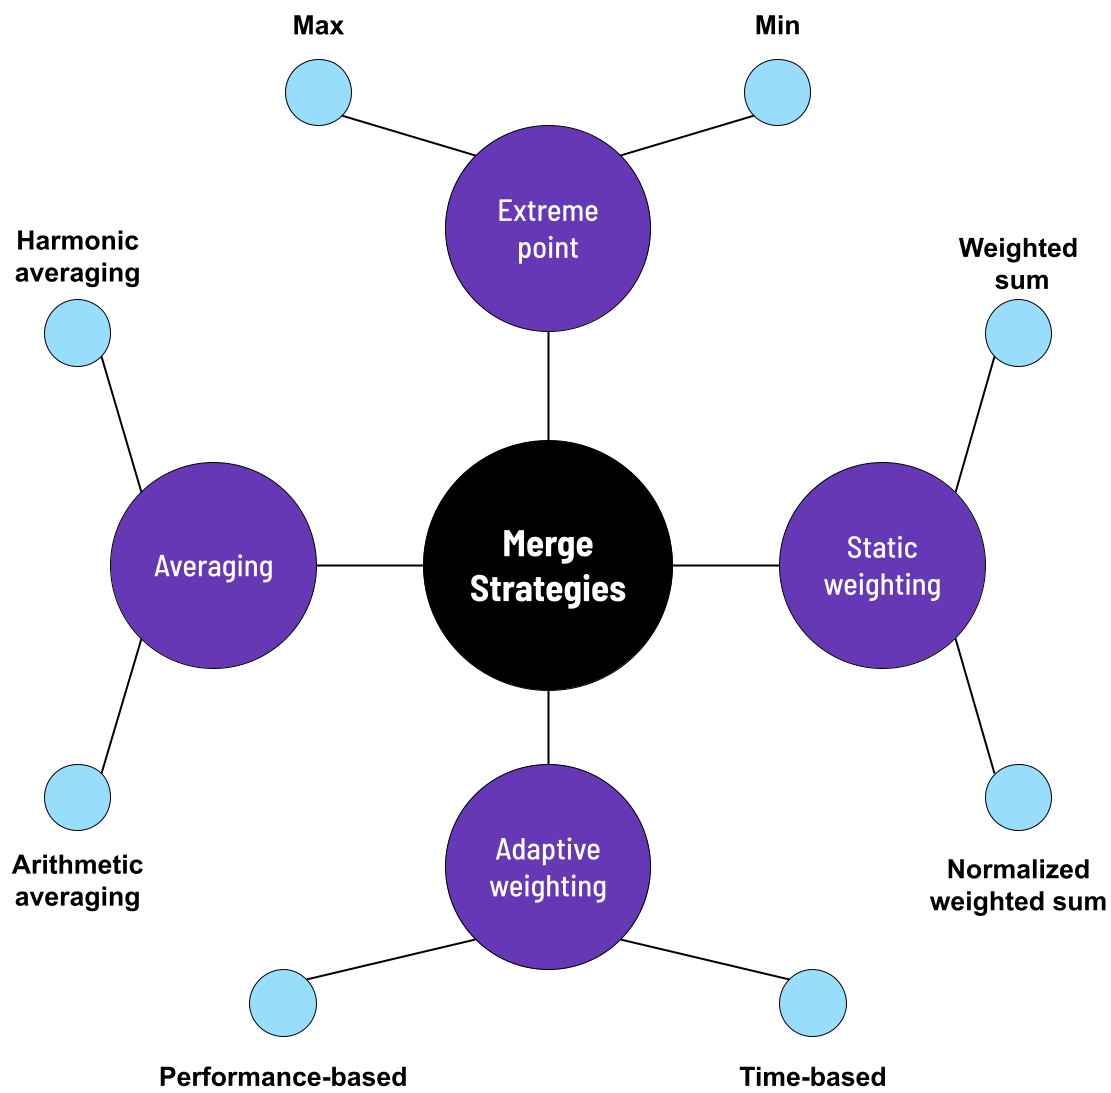
\includegraphics[width=\imgWidthL]{images/MergeStrategies.png}
  \caption[Merging strategies]{Illustration of different loss merging strategies used to merge the different loss combinations listed in \ref{tab:loss_combinations}. The objective is to identify an optimal combination for a given dataset, ultimately enhancing the model's performance.}
  \label{merging_strategies}
\end{figure}

\subsubsection*{Extreme Point}
This section introduces two extreme point strategies, the Max and the Min strategies, which aim to prioritize the largest or smallest value from different loss outputs.

\textbf{\emph{The Max strategy (MAX)}} strategy calculates the loss as the maximum value among the distribution-based, region-based, and boundary-based losses. This approach aims to prioritize the most significant loss at each training step, focusing on the most challenging examples and improving overall performance. However, one disadvantage of this method is that it may focus exclusively on one loss if the range of losses is significantly different. This might lead to an unbalanced approach that fails to consider all losses during model training appropriately. Formally the loss is defined as:
\begin{equation}
  L_{MAX} = \max_{i=1,\dots,n} L_i
  \label{eqn:max_strategy}
\end{equation}
This equation shows that the Max strategy selects the maximum loss value, denoted as $L_{MAX}$, from a set of $n$ losses, $L_1$ through $L_n$.

\textbf{\emph{The Min strategy (MIN)}} takes the minimum value of the three loss functions at each training step and uses it for gradient updates. While this strategy can provide smooth convergence by focusing on the best-performing loss, it may overlook more significant errors in other losses and lead to suboptimal performance. It is defined as:
\begin{equation}
  L_{MIN} = \min_{i=1,\dots,n} L_i
\end{equation}
where the minimum value $L_{MIN}$ is selected from a set of $n$ losses, $l_1$ through $L_n$.
\subsubsection*{Averaging}
Numerous mathematical techniques exist for determining the average of $n$ data points, where, in this context, the data points represent $n$ losses denoted as $L_1, L_2, \dots, L_n$. This study focuses on two prominent averaging strategies, which are discussed below.

\textbf{\emph{Arithmetic averaging (AVG)}} is based on the arithmetic mean considering the average value of the individual loss functions as a final loss. This approach aims to balance the weight of each loss function and can provide a good trade-off between the best and worst-performing results. However, one disadvantage of this method is that critical information could be smoothed out, causing the model to miss essential properties of the data.

The averaging strategy is formally defined as:

\begin{equation}
  L_{AVG} = \frac{1}{n} \sum_{i=1}^{n} L_i
\end{equation}

This equation shows that the averaging strategy calculates the average arithmetic loss, denoted as $L_{AA}$, from a set of $n$ losses, $L_1$ through $L_n$.

\textbf{\emph{Harmonic averaging (HARMONIC)}} is a technique to form an average by dividing the number of data points by the sum of the reciprocals of the data points. The harmonic mean is typically used for rates and ratios such as speed, fuel efficiency, or price-to-earnings ratios. It is also applicable to merge losses specifically because it is less sensitive to outliers by down-weighting larger loss values.

The harmonic average can be formally defined as:

\begin{equation}
  L_{HARMONIC} = \frac{n}{\sum_{i=1}^{n} \frac{1}{L_i}}
\end{equation}

where $L_{HA}$ is the final harmonic average calculated from a set of $n$ losses, $L_1$ through $L_n$.
\subsubsection*{Static Weighting}
\textbf{\emph{Weighted sum (WS)}}  merging is a technique that assigns different weights to individual loss functions and then computes the sum. While this strategy is quite flexible, allowing the user to control the importance of each loss individually, it can be challenging to find the right combination without in-depth domain knowledge.

The weighted sum strategy can be formally defined as:

\begin{equation}
  L_{WS} = \sum_{i=1}^{n} w_i L_i
\end{equation}

This equation shows that the weighted sum strategy calculates the weighted sum loss value, denoted as $L_{WS}$, from a set of $n$ losses, $L_1$ through $L_n$, where $w_i$ represents the weight assigned to each loss.

\textbf{\emph{Normalized weighted sum (NWS)}} is a variation of the regular weighted sum strategy. The difference is that it outputs smaller values as the regular weighted sum as its weights get normalized, adding up to one. The proportional contribution of each weight is the same. One advantage of the normalized weighted sum is its simplicity, which lies in the weight contributions being limited to values between 0 and 1. The mathematical function that defines the normalized weighted sum is straightforward, making it a practical and accessible approach. The formula for the normalized weighted sum strategy is:
\begin{equation}
  L_{NWS} = \sum_{i=1}^{n} \frac{w_i}{\sum_{j=1}^{n} w_j} L_i
\end{equation}
where $n$ is the number of loss functions, $w_i$ is the weight of the $i$-th loss function, and $L_i$ the value of the $i$th loss function.
\subsubsection*{Adaptive Weighting}
This section describes two more strategies individually designed for this project. While the first strategy's weights are crafted around the loss performance, the second strategy calculates the weights based on temporal factors such as the current training epoch or the current number of steps. Both strategies include several variations and hyperparameters, which can be set to define the weight's contribution gradually. The mathematical definition was inspired by the \acf{FL} and the Bernoulli distribution.

\textbf{\emph{Performance-based weighting (PBM)}} is a method for dynamically adapting weights depending on the performance of every single loss. The contributions of single losses to the optimization process for this method are formulated as follows:

\begin{equation}
  L_{PBM} = \sum_{i=1}^n w_i \cdot L_i
  \label{eqn:annealing}
\end{equation}

Here, $L_{PBM}$ is the performance-based loss, $L_i$ is the $i$-th component of the loss, and $w_i$ is the weight assigned to the $i$-th component.

The weight $w_i$ is calculated based on the normalized loss component $\bar{L}_i$ and a hyperparameter $\alpha$ that controls the function's slope. The following equation gives the weight $w_i$:

\begin{equation}
  w_i=(1-I)\cdot(\bar{L}_i)^{\alpha}+I\cdot(1-(\bar{L}_i))^{\alpha}
\end{equation}

Here, $I$ is a binary parameter determining whether an ascending or descending strategy is used. An ascending strategy assigns larger weights to larger losses, while a descending strategy assigns smaller weights to larger losses. The normalized loss component $\bar{L}_i$ is calculated as

\begin{equation}
  \bar{L}i=\frac{L_i}{\sum{j=1}^n L_j}
\end{equation}

where the $i$-th component of the loss is divided by the sum of all loss components, and the resulting value represents the proportion of the total loss attributed to the $i$-th component.

The choice of $\alpha$ determines the slope of the weight function, as shown in \figref{annealing}. When $I=1$, the weight function represents a descending strategy, where higher losses receive smaller weights. When $I=0$, the weight function represents an ascending strategy, where higher losses receive larger weights. By selecting appropriate values of $\alpha$, the weight function can be adjusted to achieve the desired balance between different loss components. Note that $I$ can also be set to values between $0$ and $1$. If $I=0.8$, we get a descending strategy for smaller losses and a lightly ascending strategy for larger losses.

\begin{figure}[H]%[htbp]
  \centering
  \subfigure[]{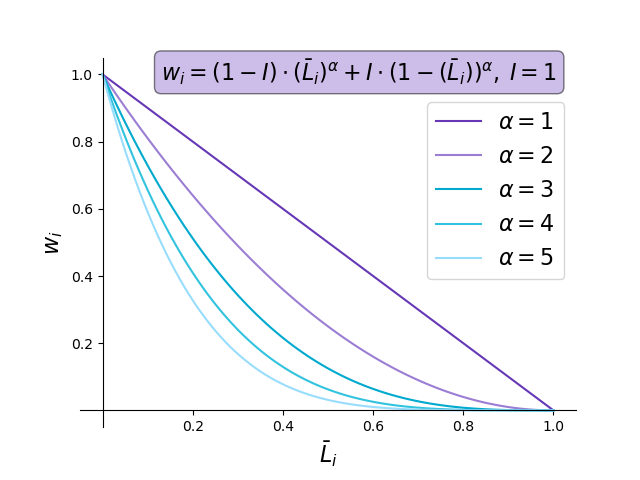
\includegraphics[width=\imgWidthTwo]{images/p_based_1.png}}
  \subfigure[]{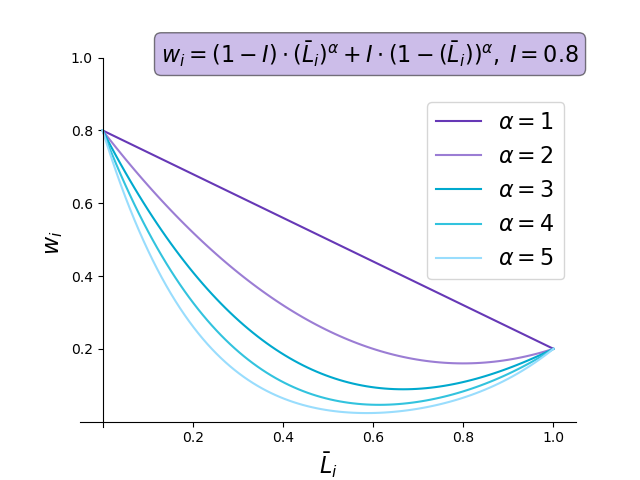
\includegraphics[width=\imgWidthTwo]{images/p_based_2.png}}\\
  \subfigure[]{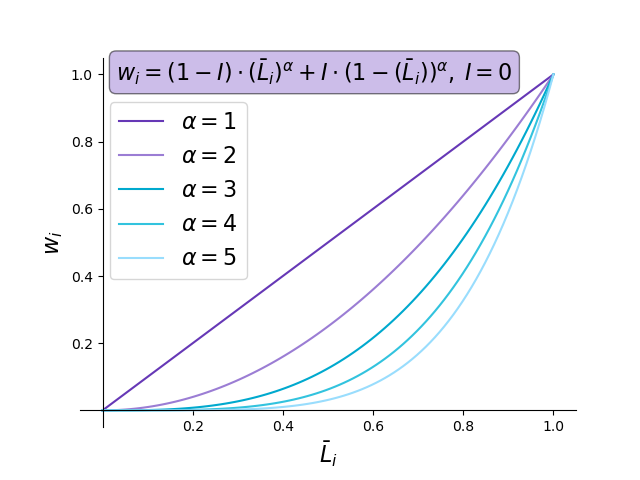
\includegraphics[width=\imgWidthTwo]{images/p_based_3.png}}
  \subfigure[]{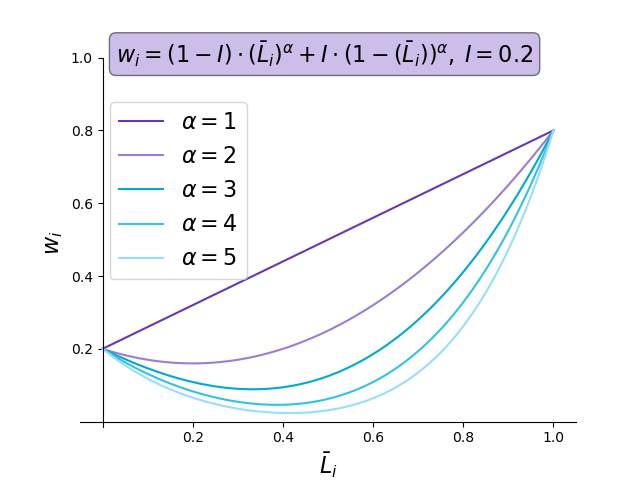
\includegraphics[width=\imgWidthTwo]{images/p_based_4.png}}
  \caption[Performance based strategy]{(a) represents the descending strategy of performance-based weighting. To use this strategy, $I$ must be set to $1$. As $\alpha$ increases, the weight contribution for larger losses decreases, while the contribution for smaller losses increases. Image (b) combines descending strategy for smaller losses and a smooth ascending strategy for larger losses. (c) represents an ascending strategy, which can be used by setting $I$ to $0$ and using $\alpha$ to control $w_i$ given a normalized loss $L_i$. In this strategy, higher losses receive higher weight proportions than smaller losses. Graph (d), opposite graph (b), represents a smooth descending strategy for smaller losses and an ascending strategy for larger losses.}
  \label{annealing}
\end{figure}

%\left(1-I\right)\cdot x^{a}+I\cdot\left(1-x\right)^{a} DESMOS

\textbf{\emph{Time-based weighting (TBM)}} is a strategy incorporating a time component to the loss calculation. The idea is to either gradually increase or decrease weights over time. The following method is implemented to be compatible with any other loss merging method discussed so far by simply adding a time-based weighting factor $u_i$ to the general weighting scheme $L_i \cdot w_i$. The function can be formally described as follows:
\begin{equation}
  L_{TBM}(t) = \sum_{i=1}^{n} w_i L_i u_i(t)
\end{equation}
where $w_i$ and $L_i$ represent the weight and loss function, respectively, of any loss functions discussed previously, and $u_i(t)$ is defined as:
\begin{equation}
  u_i(t)=
  \begin{cases}
    (1-I_i)\cdot \left(\frac{t}{T}\right)^{\alpha} + I_i \cdot\left(1-\frac{t}{T}\right)^{\alpha}, & i=1 \\
    (1-I_i)\cdot \left(\frac{t}{T}\right)^{\beta} + I_i \cdot\left(1-\frac{t}{T}\right)^{\beta},   & i=2 \\
    (1-I_i)\cdot \left(\frac{t}{T}\right)^{\gamma} + I_i \cdot\left(1-\frac{t}{T}\right)^{\gamma}, & i=3
  \end{cases}
\end{equation}
This formulation is very similar to the performance-based weighting scheme, which can be applied to every loss output individually. $0 \leq u_i(t) \leq 1$ represents the time-dependent weight of the $i$-th loss function at step or epoch $t$. $T$ denotes the total number of epochs or steps, and $\alpha \geq 1$, $\beta \geq 1$, and $\gamma \geq 1$ are parameters that control the impact on the corresponding loss functions. $I \in [0,1]$ determines whether an increasing or decreasing time-based strategy is employed. If $I=0$, the weight $u_i$ will increase as training progresses, whereas if $I=1$, $u_i$ will gradually decrease. Similar to the performance-based weighting scheme, it is possible to define $I$ as a continuous value between $0$ and $1$, changing the function's slope to the opposite direction using the same strategy. In other words, weights, during the beginning, could be gradually decreased and then automatically increased again when approaching the end of the training cycle.

% Please add the following required packages to your document preamble:
% \usepackage{multirow}
% \usepackage{graphicx}
% \usepackage[table,xcdraw]{xcolor}
% If you use beamer only pass "xcolor=table" option, i.e. \documentclass[xcolor=table]{beamer}
\begin{table}[H]
    \centering
    \resizebox{\textwidth}{!}{%
    \begin{tabular}{|l|l|c|l|}
    \hline
    \rowcolor[HTML]{6638B6} 
    {\color[HTML]{FFFFFF} Strategy type} &
      \multicolumn{1}{c|}{\cellcolor[HTML]{6638B6}{\color[HTML]{FFFFFF} Strategy}} &
      {\color[HTML]{FFFFFF} Hyperparameters} &
      \multicolumn{1}{c|}{\cellcolor[HTML]{6638B6}{\color[HTML]{FFFFFF} Definition}} \\ \hline
     &
      MAX &
      - &
      $\max_{i=1,\dots,n} L_i$ \\ \cline{2-4} 
    \multirow{-2}{*}{Extreme point} &
      MIN &
      - &
      $\min_{i=1,\dots,n} L_i$ \\ \hline
     &
      AVG &
      - &
      $\frac{1}{n} \sum_{i=1}^{n} L_i$ \\ \cline{2-4} 
    \multirow{-2}{*}{Averaging} &
      HARMONIC &
      - &
      $n / \sum_{i=1}^{n} \frac{1}{L_i}$ \\ \hline
     &
      WS &
      \multicolumn{1}{l|}{$w_1,w_2,...w_n$} &
      $\sum_{i=1}^{n} w_i L_i$ \\ \cline{2-4} 
    \multirow{-2}{*}{Static weighting} &
      NWS &
      \multicolumn{1}{l|}{$w_1,w_2,...w_n$} &
      $\sum_{i=1}^{n} w_i / \sum_{j=1}^{n} w_j L_i$ \\ \hline
     &
      PBM &
      \multicolumn{1}{l|}{$\alpha,I$} &
      $\sum_{i=1}^n ((1-I)\cdot(\bar{L}_i)^{\alpha}+I\cdot(1-(\bar{L}_i))^{\alpha})\cdot L_i$ \\ \cline{2-4} 
    \multirow{-2}{*}{Adaptive weighting} &
      TBM &
      \multicolumn{1}{l|}{$\alpha,\beta,\gamma,I$} &
      $\sum_{i=1}^{n} w_i L_i u_i(t)$ \\ \hline
    \end{tabular}%
    }
    \caption[Summary of loss merging strategies]{Summary of loss merging strategies including their hyperparameters}
    \label{tab:loss_merging_strategies_overview}
    \end{table}